\section{Sensitivity of the Rust Model}
\thispagestyle{plain} % surpress header on first page

As described in section \ref{generalMPEC}, the economic literature exploring the benefits of MPEC and NFXP for structural estimation is limited to studies by \cite{Su.Judd.2012}, \cite{Dube.Fox.Su.2012}, \cite{Jorgensen.2013}, \cite{Iskhakov.2016} and \cite{Dong.Hsieh.Zhang.2017}. While in these papers different economic models are considered, the set up chosen is quite clean, being mainly free of any model misspecification and allowing mostly for stable, small numerical errors in the calibration procedure. From a practical perspective and in a research setting where economic models and calibration procedures become more complex, their comparison of MPEC and NFXP is inherently limited to a world in which the modeling and calibration procedure is performed with a minimal error. In a more realistic set up that practioners commonly face where their mathematical model might be more or less off from reality and the computational model has to work with many approximations, there might actually be a larger difference between the two approaches. The previously mentioned studies comparing the two approaches unanimously find that the qualitative results, i.e. the parameter estimates are the same for both and focus on the implementation side covering the speed and rate of convergence. The idea of my following simulation study is to break with the clean comparison of MPEC and NFXP by deliberately introducing some numerical error and model misspecification to test how the two approaches react to it. In this comparison I focus on qualitative aspects investigating how well the two approaches recover the true underlying model. For this a first aspect of the UQ framework comes into play. As I will also change the level of model misspecification in the Rust model a naive comparison of how the structural parameters of the underlying data generating process are recovered, as done by \cite{Su.Judd.2012}, is flawed. Therefore I rely on the previously used QoI of the counterfactual demand level at replacement cost of 11,000 Dollars. This quantity can be calculated and compared no matter the degree of model misspecification and it is an indicator on how well certain parameters in combination with some model and numerical specifications actually uncovers the predictions of the true underlying model and data generating process. A second aspect from uncertainty quantification entering my following simulation study is the general framework of \cite{Oberkampf.2010}. They devise an approach for scientific computing in which they account for model and numerical error as well as parameter uncertainty and propagate them in various combinations through a model. This results in many different distributions of a QoI that in the end is visualized such that it is informative about the uncertainty in the QoI for those that intend to actually use the model outcome. In my simulation study I pick up key ideas of this framework and consequently investigate how changes in model specification and numerical implementation in the calibration procedure translate into the distribution of a QoI and hence its uncertainty. I do so by performing a large scale Monte Carlo simulation for the previously described Rust model. The model is well explored and can therefore be seen as the perfect benchmark for such a study whose results might probably be taken as a lower bound for the effects found of such a simulation in modern and much more complex structural models.

\subsection{The Simulation Setup}

The setup for my simulation study is inspired by that found in \cite{Iskhakov.2016}. Consequently, I stay close to the data generating process and ideas explored in section \ref{generalsetup}. First of all, I simulate 250 data sets based on the following true data generating process. The discount factor $\beta$ equals to 0.975 and the cost function $c(.)$ is linear with a scale parameter of $10^{-3}$, i.e. $c(x; \theta_{11}) = 0.001 \times \theta_{11} x$. The true cost parameters are:

\begin{equation*}
\begin{split}
& RC = 11.7257 \\
& \theta_{11} = 2.4569 . \\
\end{split}
\end{equation*}

This parametrization follows exactly the one already encountered before. The first change enters with the true transition probabilities. This change is necessary due to the nature of how the simulation of data is implemented in the ruspy package. The package gives out a data set in which the mileage state of a bus is already discretized according to a previously specified grid size. As a reminder this grid size was set to 175 in the previous setup. In this simulation I intend to investigate how a different discretization of the mileage in the same data set leads to changes in the calibration and later in the QoI. To preserve the information in the data set I have to simulate the data with a large grid size and then derive the same data set with lower grid size from it. I choose to set the grid size to 400 for the initial data generation. The previous parametrization of section \ref{generalsetup} that is optimized for a grid size of 175 will yield unproportionally small variation in mileage when used for my increased grid size. Accounting for this I adjust the true transition probabilities to be the following:

\begin{equation*}
	\resizebox{.9\hsize}{!}{$\theta_3 = \begin{pmatrix}
		0.04685 & 0.04685 & 0.22375 & 0.22375 & 0.22295	& 0.22295 & 0.00635 & 0.00635 & 0.0001 & 0.0001
		\end{pmatrix}.$}
\end{equation*}

From those 250 data sets with grid size 400 I now derive the same data sets with decreased grid size of 200 and 100. These data sets are calibrated with different specifications which will yield different estimated parametrizations and parameters that might cause different predictions of the QoI. Before I will explain which dimensions of the calibration procedure are tweaked, let us check on how this relates to the UQ framework from before.

As was already described the mathematical model $f(\theta)$ is the demand function in equation \ref{eq19} which in turn depends on how the Rust model is specified in order to obtain the choice probabilities $P(d|x; \theta)$ and the transition probabilities $p_3(x'|x, d; \theta_3)$ (see equation \ref{eq18}). When taking for granted that the general setup of the Rust model and its assumptions are warranted, there are several ways to easily specify the model differently which would result in changes of the two probabilities. As in the UQ framework, there might be uncertainty about the mathematical model itself which can be captured by varying functional forms of the cost function. Above that, there is uncertainty about how the parameters $\beta$ as well as $\theta$ actually look like. This is further complicated by the fact that the model does not allow us to estimate $\beta$. This leaves us quite uninformed about which $\beta$ and cost function to employ to actually explain some given data. Those circumstances already induced \cite{Rust.1987} to estimate the model several times using different specifications. In this sense my simulation will be a natural extension of his explorations. Apart from the previously explained sources of model and parameter uncertainty, there still remains variation in the model outcome stemming from the numerical implementation of the mathematical model, i.e. from the exact specification of how to solve equation \ref{eq18} with a computational model. All those sources and their effect I will account for in my simulation to a certain degree. My approach will deviate from the typical workflow in UQ, though, in some ways. Usually in uncertainty quantification (compare \cite{Smith.2013, Oberkampf.2010}) there is already some prior knowledge on how the distribution of the parameters of the model look like. This distribution is then propagated through each combination of plausible mathematical model and computational model specification. This results in a probability distribution of a QoI for each mathematical-computation-model-combination specified. In my setup, it is ad-hoc not clear how a possible distribution of the parameter vector $\theta$ might look like. Another factor is that the distribution worth propagating through the model also depends on how the mathematical and computational model are specified as the parameters are calibrated using data and a certain specification that later also affects the specification of the demand function. Another factor that is not linked directly to the demand function but potentially affects the calibration procedure and hence the plausible distribution of $\theta$ is the choice of MPEC or NFXP. This remains to be shown, though. Resting on the previous discussion, my approach can be summarized like the following. I combine possible errors in the mathematical and computational representation in the Rust model. These errors directly affect the demand function by itself and further do so indirectly by different calibration results that yield plausible, varying distributions of $\theta$ that affect the QoI. I further add another source of parameter uncertainty that stems from the calibration procedure itself and hence only changes the QoI through the variation in parameters. I test two possible numerical errors which are the difference in using either MPEC or NFXP as well as relying on numerical first order derivatives for the likelihood function as opposed to analytical ones. By this I perform an uncertainty quantification of the Rust model in which I incorporate different sources of error and in which the only information on the parametrization of the model comes from the model itself through its calibration. The goal of the approach is twofold. It shall uncover whether NFXP and MPEC might yield different qualitative results when facing unfavourable conditions while at the same time perform a broader check of the model implications when facing reasonable discrepancies in the mathematical and numerical model specification. Hence, it is supposed to be a comprehensive approach that gives as much valuable information to policy makers as possible. \paragraph{}

I will now explain the exact steps taken to arrive at the results presented below. I run a Monte Carlos simulation with 250 runs each per specification. As a benchmark case I estimate the parameters when relying on the true specification of the model. This means that I run the estimation on the 250 data sets with gird size 400, linear cost function, a $\beta$ of 0.975 as well as analytical first order derivatives of the likelihood function. This first specification I call the "correctly specified" in the following. This and all the other specifications are hence estimated on 250 data sets and this once per approach MPEC and NFXP. This simulation is equivalent to a parametric bootstrap, as noted by \cite{Su.Judd.2012}, which allows me to obtain sample statistics for the parameters. While the 250 runs do not allow me to obtain exactly unbiased estimates of the true parameters, I still do not opt for more runs as the sheer amount of different specifications I consider would make it too computationally expensive given the limited time during my thesis. Further it makes it more comparable to the set up in \cite{Iskhakov.2016} and \cite{Su.Judd.2012} as they also solely simulated 250 data sets per specification. Due to estimating the model twice (once with MPEC and once with NFXP) per specification 500 runs are performed. So which specifications do I use? The specifications differ in the degree of model misspecification (or flexibility) and numerical error. The model uncertainty is introduced by allowing more flexibility in the cost function than the true data generating process actually displays. The true cost function is linear but I also allow the optimizers to employ more flexible cost function. Specifically, quadratic cost $c(x; \theta_{11}, \theta_{12}) = \theta_{11}x + \theta_{12}x^2$ or cubic cost $c(x; \theta_{11}, \theta_{12}, \theta_{13}) = \theta_{11}x + \theta_{12}x^2 + \theta_{13}x^3$ are possible. Additionally, I add the dimension of a wrongly specified $\beta$. In my setup it is therefore possible that the estimation is based on $\beta = 0.985$ although it is actually equal to 0.975.

A numerical error is introduced in two ways. While the true data generating process conveys all its information on the mileage state into a grid of 400 points, I deliberately estimate the model parameters with some loss of this information. As already mentioned, this is accounted for by running the calibration after discretizing the mileage state further from 400 to either 200 or 100 grid points. Lastly, I give the option of the realistic feature that the economic model and the estimation procedure give rise to a likelihood function that has to rely on numerical first order derivatives as opposed to analytical ones. This is the only part of the specifications that affects the QoI solely through the calibration of the structural parameters.

Clearly, it might be possible that several of those misspecifications occur at the same time and that the uncertainty introduced in the QoI might depend on this. For that reason, I build the Cartesian product of all those single misspecifications to estimate each of its possible combinations which leaves me with 36 specifications for which I separately estimate the parameters for 250 data sets using the NFXP and MPEC, respectively. A list of all specifications can be found in Table \ref{table4} in the appendix B. All this amounts to 18,000 runs for which the model is calibrated and the resulting parameters are taken to calculate the expected implied demand for bus engines for the counterfactual level of replacement cost at 11,000 Dollars. Selected results of this procedure are presented in the following section.

\subsection{The Results}

In the first step, we look at some partial sensitivity explorations to get a sense of how the QoI reacts to small changes in the model setup. This means that at first I only look at those specifications in which I deviate from the correctly specified model in only one dimension. This is I am either tweaking the model dimension, i.e. just the cost function and/ or $\beta$ or I change the numerical dimension consisting of the grid size and the use of numerical gradients. Before I do so let us fill up on one missing ingredient of the setup discussion from before. The setup for MPEC is exactly chosen as it was described in section \ref{generalsetup}. Again I use IPOPT as a solver with the tolerances specified as before. My initial intention to keep the setup as close to the one in \cite{Iskhakov.2016} as possible had to be eased a bit for the NFXP, though. This is due to malperformance of the initial setup that I employ to replicate the results in \cite{Iskhakov.2016} when facing more flexible cost functions. This will be the starting point of the following section.

\subsubsection{The Partial Perspective}

\begin{figure}[!b]
	\caption{The QoI when varying the Cost Function}
	\vspace*{-4mm}
	\centering
	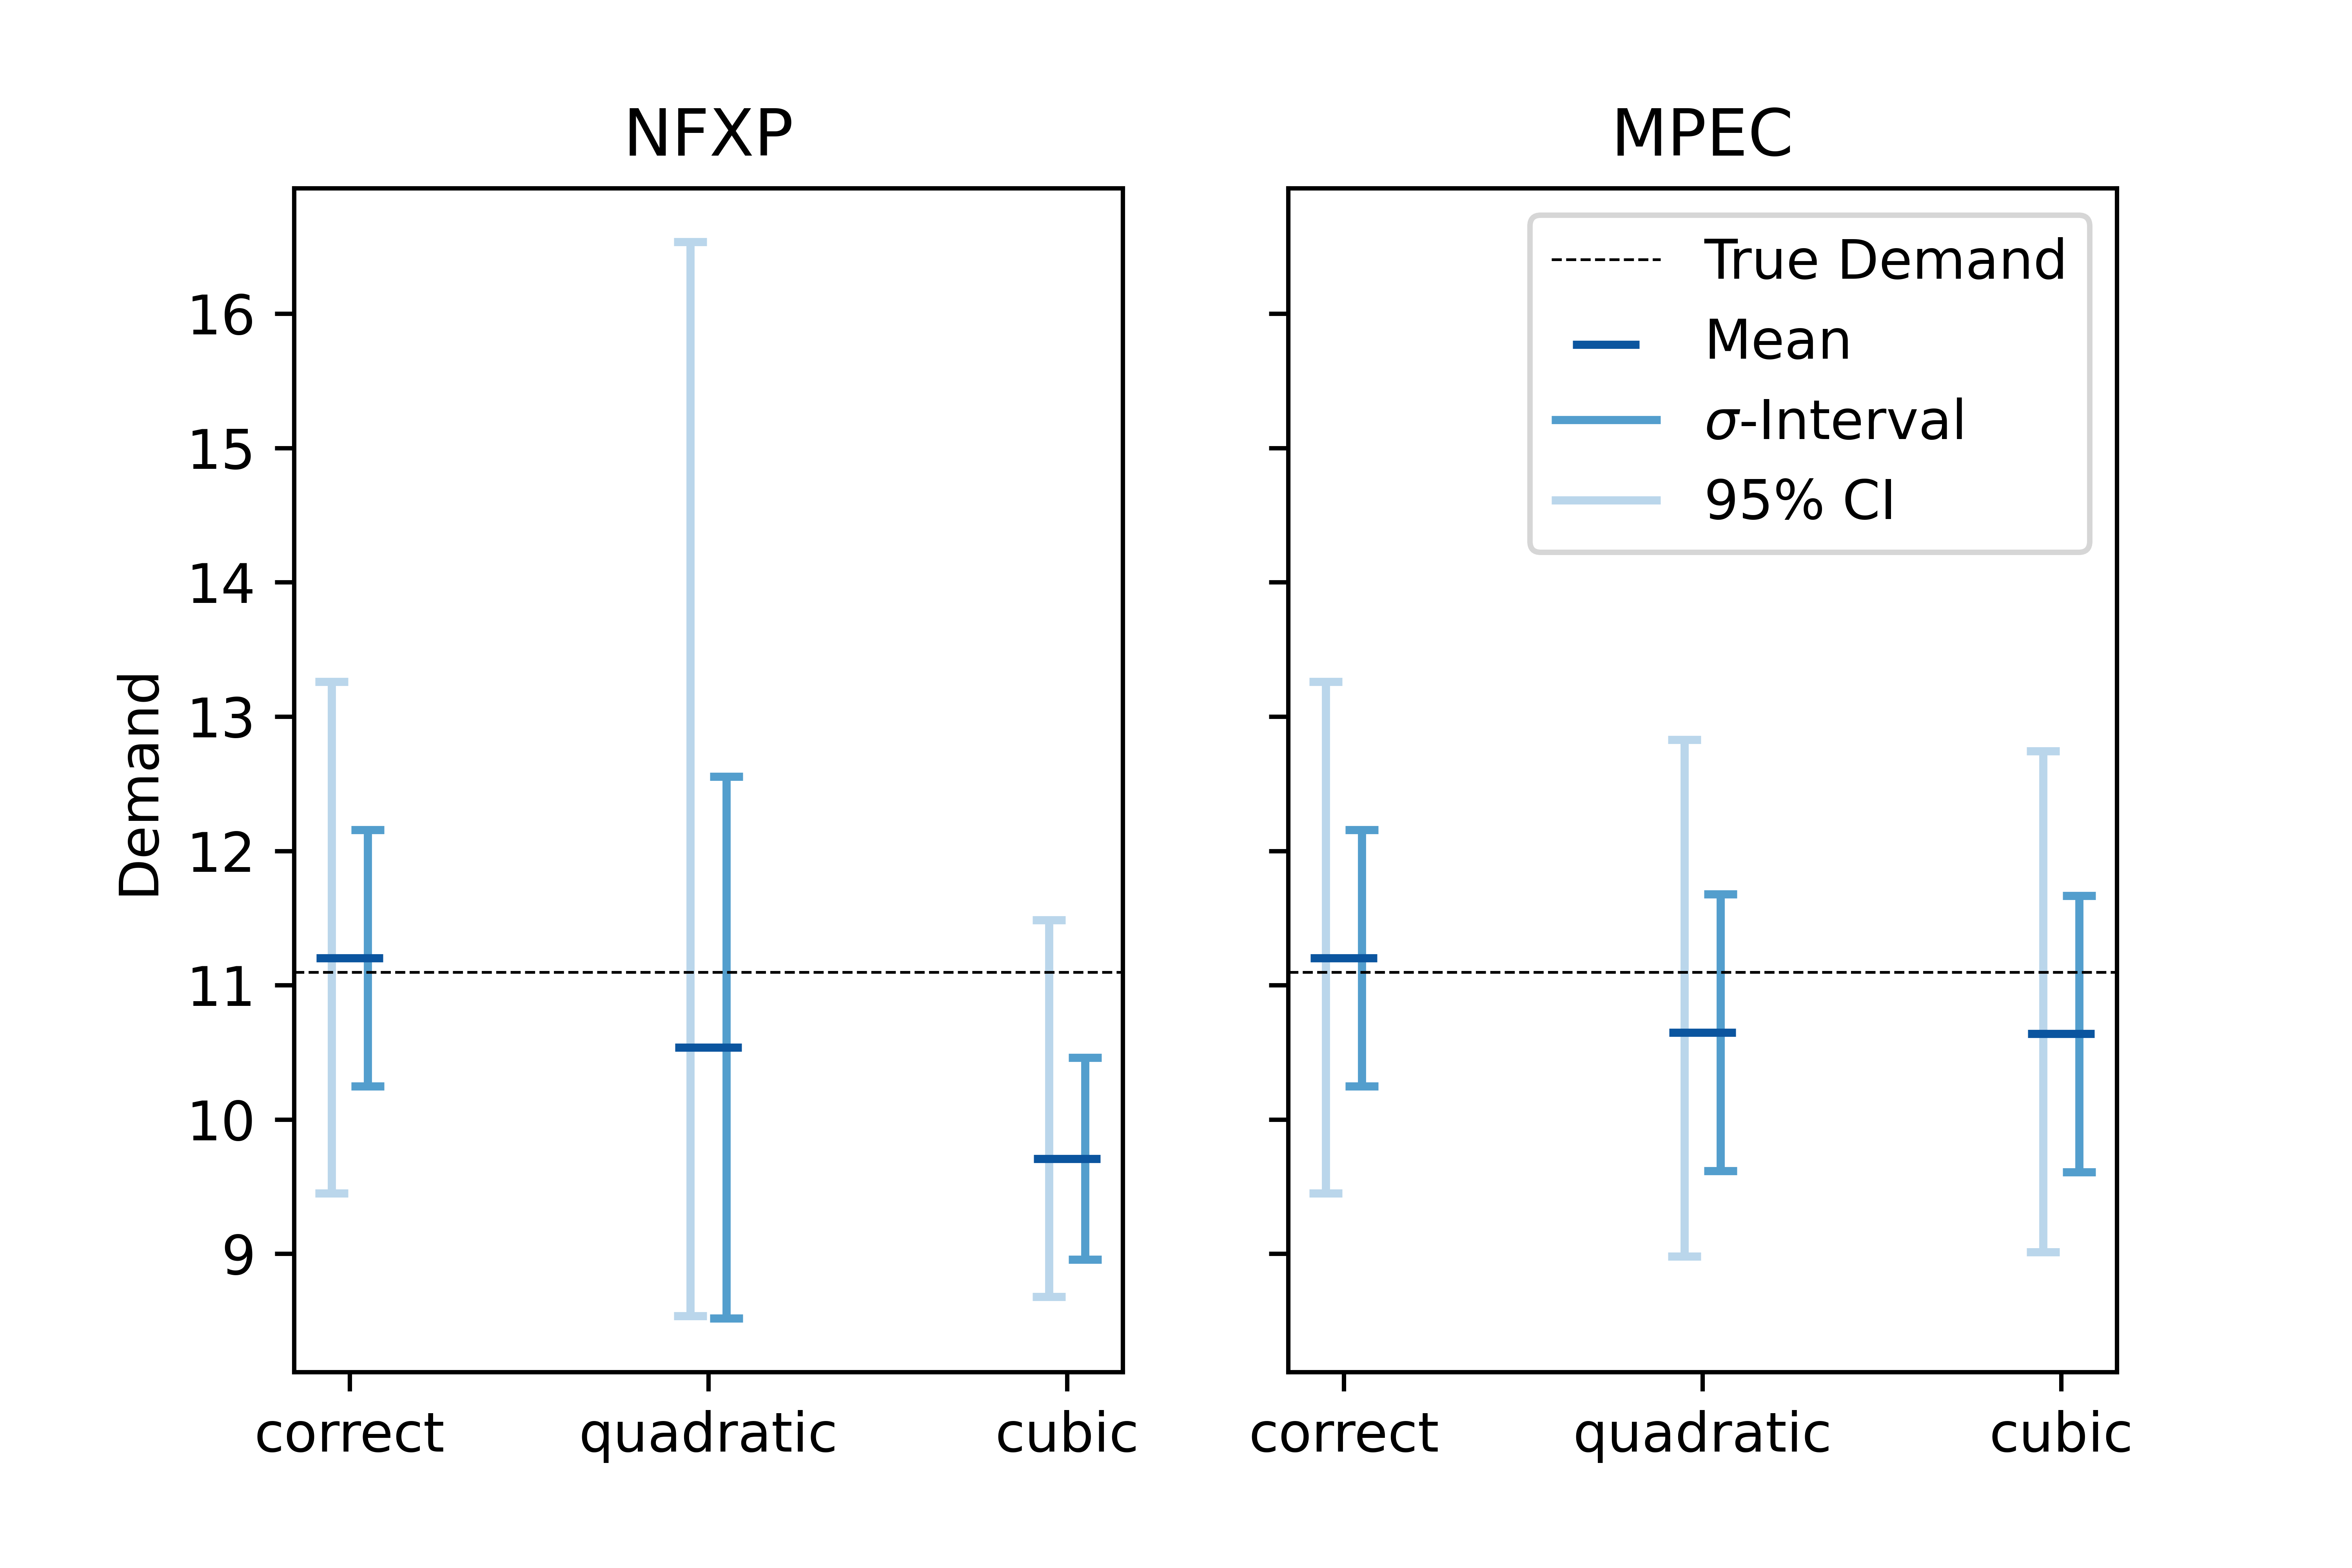
\includegraphics[scale=0.9]{../figures/figure_5.png}
	\label{figure5}
\end{figure}

The first results are those coming from the specifications in which I only add more flexibility to the cost functions than are used to calibrate the Rust model. Apart from that the model stays correctly specified. In Figure \ref{figure5}, I present some summary statistics for the QoI depending on which specification is used for NFXP and MPEC separately. This same kind of figure with its labeling will follow us along for several explorations which is why the legend in the subsequent figures will be dropped. Figure \ref{figure5} shows the correctly specified model at the very left as a benchmark case for both NFXP and MPEC. For this and the other specifications the mean of the QoI across the 250 runs, as well as its 95\% confidence and standard deviation interval are reported.\footnote{For the bootstrap confidence interval the percentile bootstrap is used (compare \cite{Davison.1997} chapter 5).} As already noted before the mean of the QoI for the correctly specified model does not exactly match the true value of the QoI. This is the case as there are not sufficiently many Monte Carlo runs such that the mean of the structural parameters are estimated with some small sample bias which translates into the QoI. As a reminder the true QoI is derived from the true underlying model and its true structural parameters. In our setting the true QoI is the following:

\begin{equation*}
	QoI_{true} = 11.095.
\end{equation*}

When using the correctly specified model, as expected, NFXP and MPEC yield virtually the same results for all three key statistics. The mean comes in at $11.203$ while the one standard deviation interval spreads from $10.248$ to $12.157$ with the confidence interval being equal to $(9.449, 13.261)$. In the nest specification to the right the correct model is maintained with the exception that the calibration procedure now assumes the cost function to be more flexible by adding a possible quadratic term. This reveals an interesting difference between the NFXP and MPEC which I tried to eliminate but could not entirely. Firstly, the means for the QoI for both approaches now underestimate the true one while the NFXP does so more strongly than MPEC. NFXP yields $10.537$ while MPEC estimates $10.646$. This difference stems from different estimates for all three structural cost parameters. Both approaches have a convergence rate of 100 percent but when comparing the estimates per run one can observe that the two approaches systematically find different solutions in every run. The NFXP implementation that yields these results is actually obtained by using the scipy implementation of the L-BFGS-B (see \cite{Byrd.1997} and \cite{scipy.2020}) with its default tolerances. Apart from that the setup of the NFXP algorithm used here is the same as in section \ref{generalsetup}. Solely I replace the BHHH by the above mentioned solver.\footnote{In an initial try I ran the whole simulation with the BHHH with the tolerances exactly set to the ones from section \ref{generalsetup}. This produced the results in Figure \ref{figure12} which are very far off. I first tried to allow for a more precise fixed point calculation by setting the maximum number of contraction and N-K iterations each from 20 to 40. This only altered the results marginally. In a second step I tried some combinations of relative and absolute tolerances: Specifically, from $(10^{-3}, 10^{-6})$ to $(10^{-13}, 10^{-16})$ in steps of increasing exponent of two. Again, it did not change the results so I switched to the L-BFGS-B. When using that one as well, the results do not change substantially when varying the tolerances which is why in the end I simply adapt the default settings for the optimizer and the tolerances from section \ref{generalsetup} for the fixed point calculation. I experimented with tolerance ranging from $10^{-3}$ to $10^{-21}$.} The figure further reveals that the variation in estimates for the QoI is a lot larger when relying on the NFXP as opposed to MPEC. This pattern seems to flip around, though, when assuming the cost function to have a cubic form. The underestimation of the QoI in the case of NFXP becomes even more pronounced, while all key statistics stay roughly constant when applying MPEC.

This qualitative difference between the two approaches is surprising as they theoretically both solve the same problem and find the same results as proven by \cite{Su.Judd.2012}. In practice, though, the calibration procedure in the Rust model cannot be solved analytically and hence different problem formulations can react differently on numerical solving. A further complicating factor is posed by the use of different optimizers for the two approaches. Internally, their functioning clearly differs as for instance both rely in my case on a numerical approximation of the Hessian matrix which already differs analytically due to the competing problem formulations but will even differ more due to contrasting approximation techniques. It is entirely possible that despite my extensive experimentation with tolerances, the NFXP can be set up such that it obtains the same results as MPEC in my specifications. At the same time, though, as the two approaches are promoted as competitors as opposed to complements, many practioners most likely rely on only either of the two approaches which will possibly leave them with the single results of MPEC or NFXP as I found them. Clearly, looking separately at them, they both do not appear implausible. Yet, having estimated the other approach as well would convey additional information about the quality of the other.

\begin{figure}[!b]
	\caption{The QoI when varying $\beta$ and the Cost Function}
	\vspace*{-4mm}
	\centering
	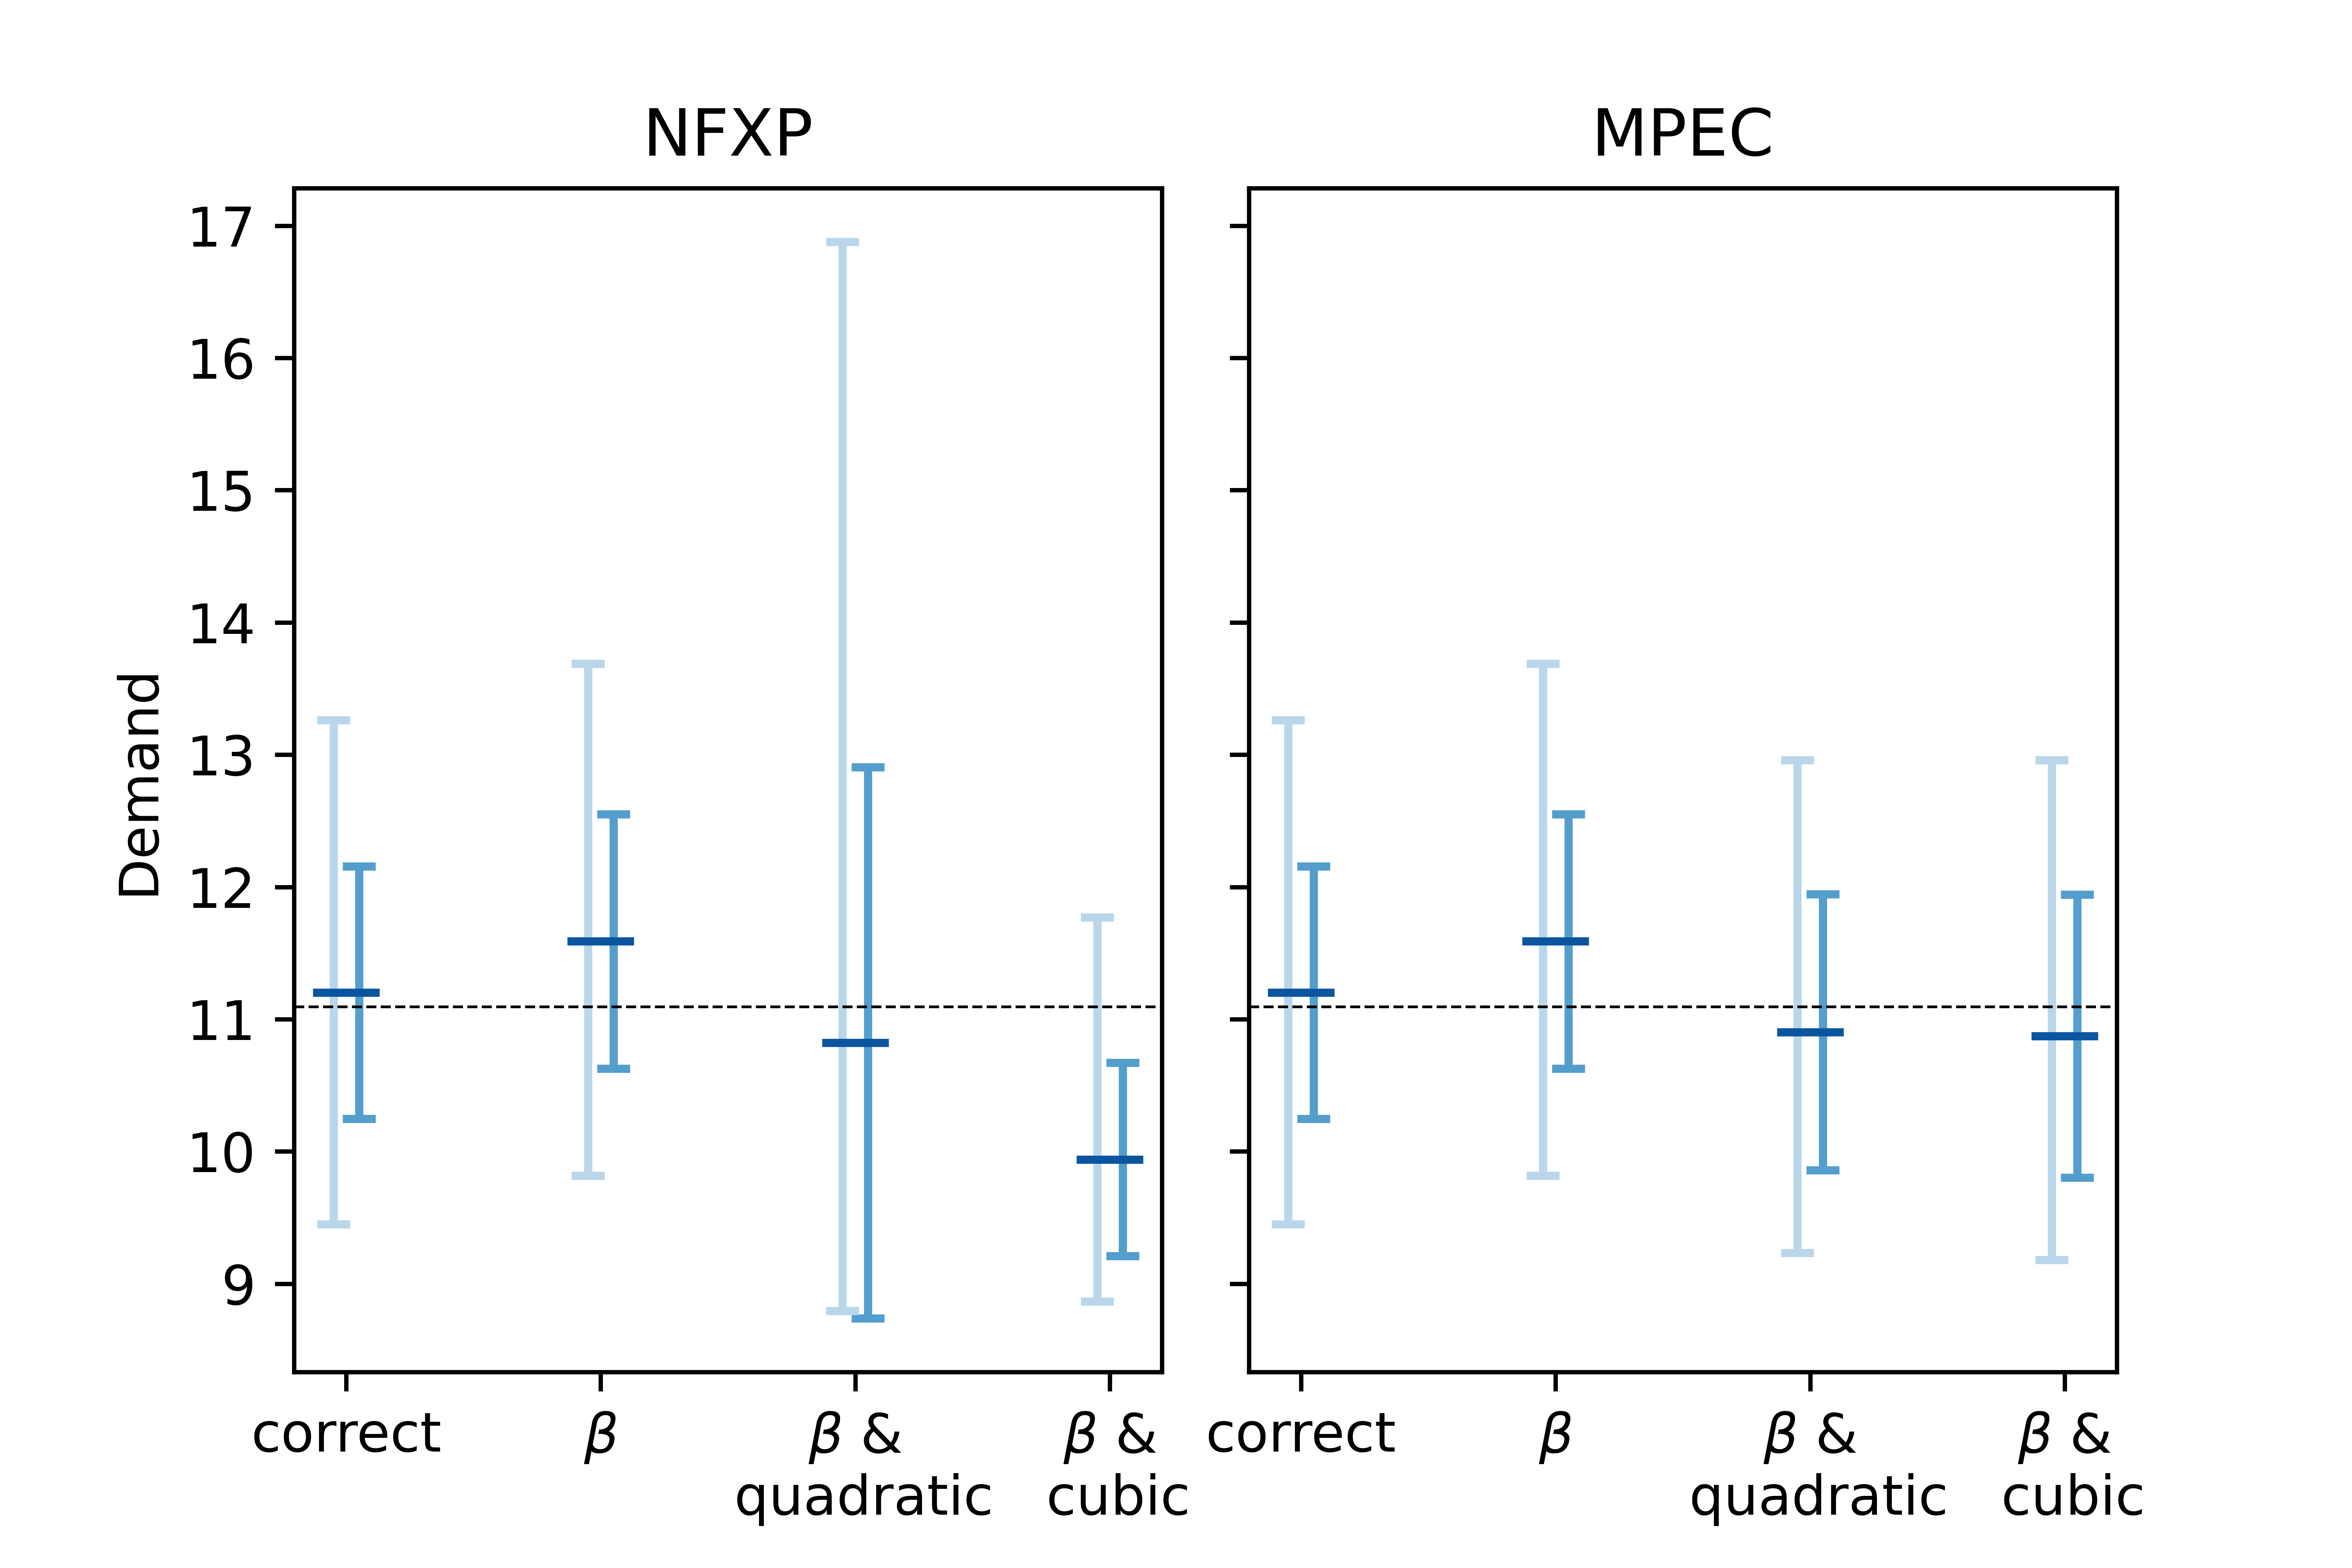
\includegraphics[scale=0.9]{../figures/figure_6.png}
	\label{figure6}
\end{figure}

From an uncertainty perspective it is interesting to note that giving more flexibility in the cost function to the estimation procedure does not cause the solver to simply estimate linear cost but rather exploit the two additional terms in the cost function. This results in a downward bias for the QoI irrespective of using the NFXP or MPEC. Looking at MPEC alone, it seemingly shifts the distribution of the QoI.

In Figure \ref{figure6}, the second part of the model dimension is tweaked. In a first step, the solver is given the information that the true $\beta$ is assumed to be equal to 0.985. This leads for both MPEC and NFXP to an overestimation of the QoI in the exact same way. The mean increases now to $11.588$. In the next step, I incorporate the first interaction of misspecifications. To the wrongly specified $\beta$ more flexibility in the cost function is added to cover all possible cases of model misspecification in my setup. As already observed in the singular view of just a change in the cost function, the increased flexibility causes the mean estimates to be shifted downwards again. This change happens in a very similar magnitude as it did in Figure \ref{figure5} with $\beta$ being equal to 0.975. Interestingly, the predictions when employing misspecification in $\beta$ and more flexibility than needed in the cost function are improved in comparison to misspecification in only one of those two dimensions. At least when only facing model error, in my example, an increased error yields better results as the two errors balance each other out. It is further worth mentioning that in all of the so far considered specifications, every run converges irrespective of NFXP or MPEC. \paragraph{}

\begin{figure}[!b]
	\caption{The QoI when varying the Grid Size}
	\vspace*{-4mm}
	\centering
	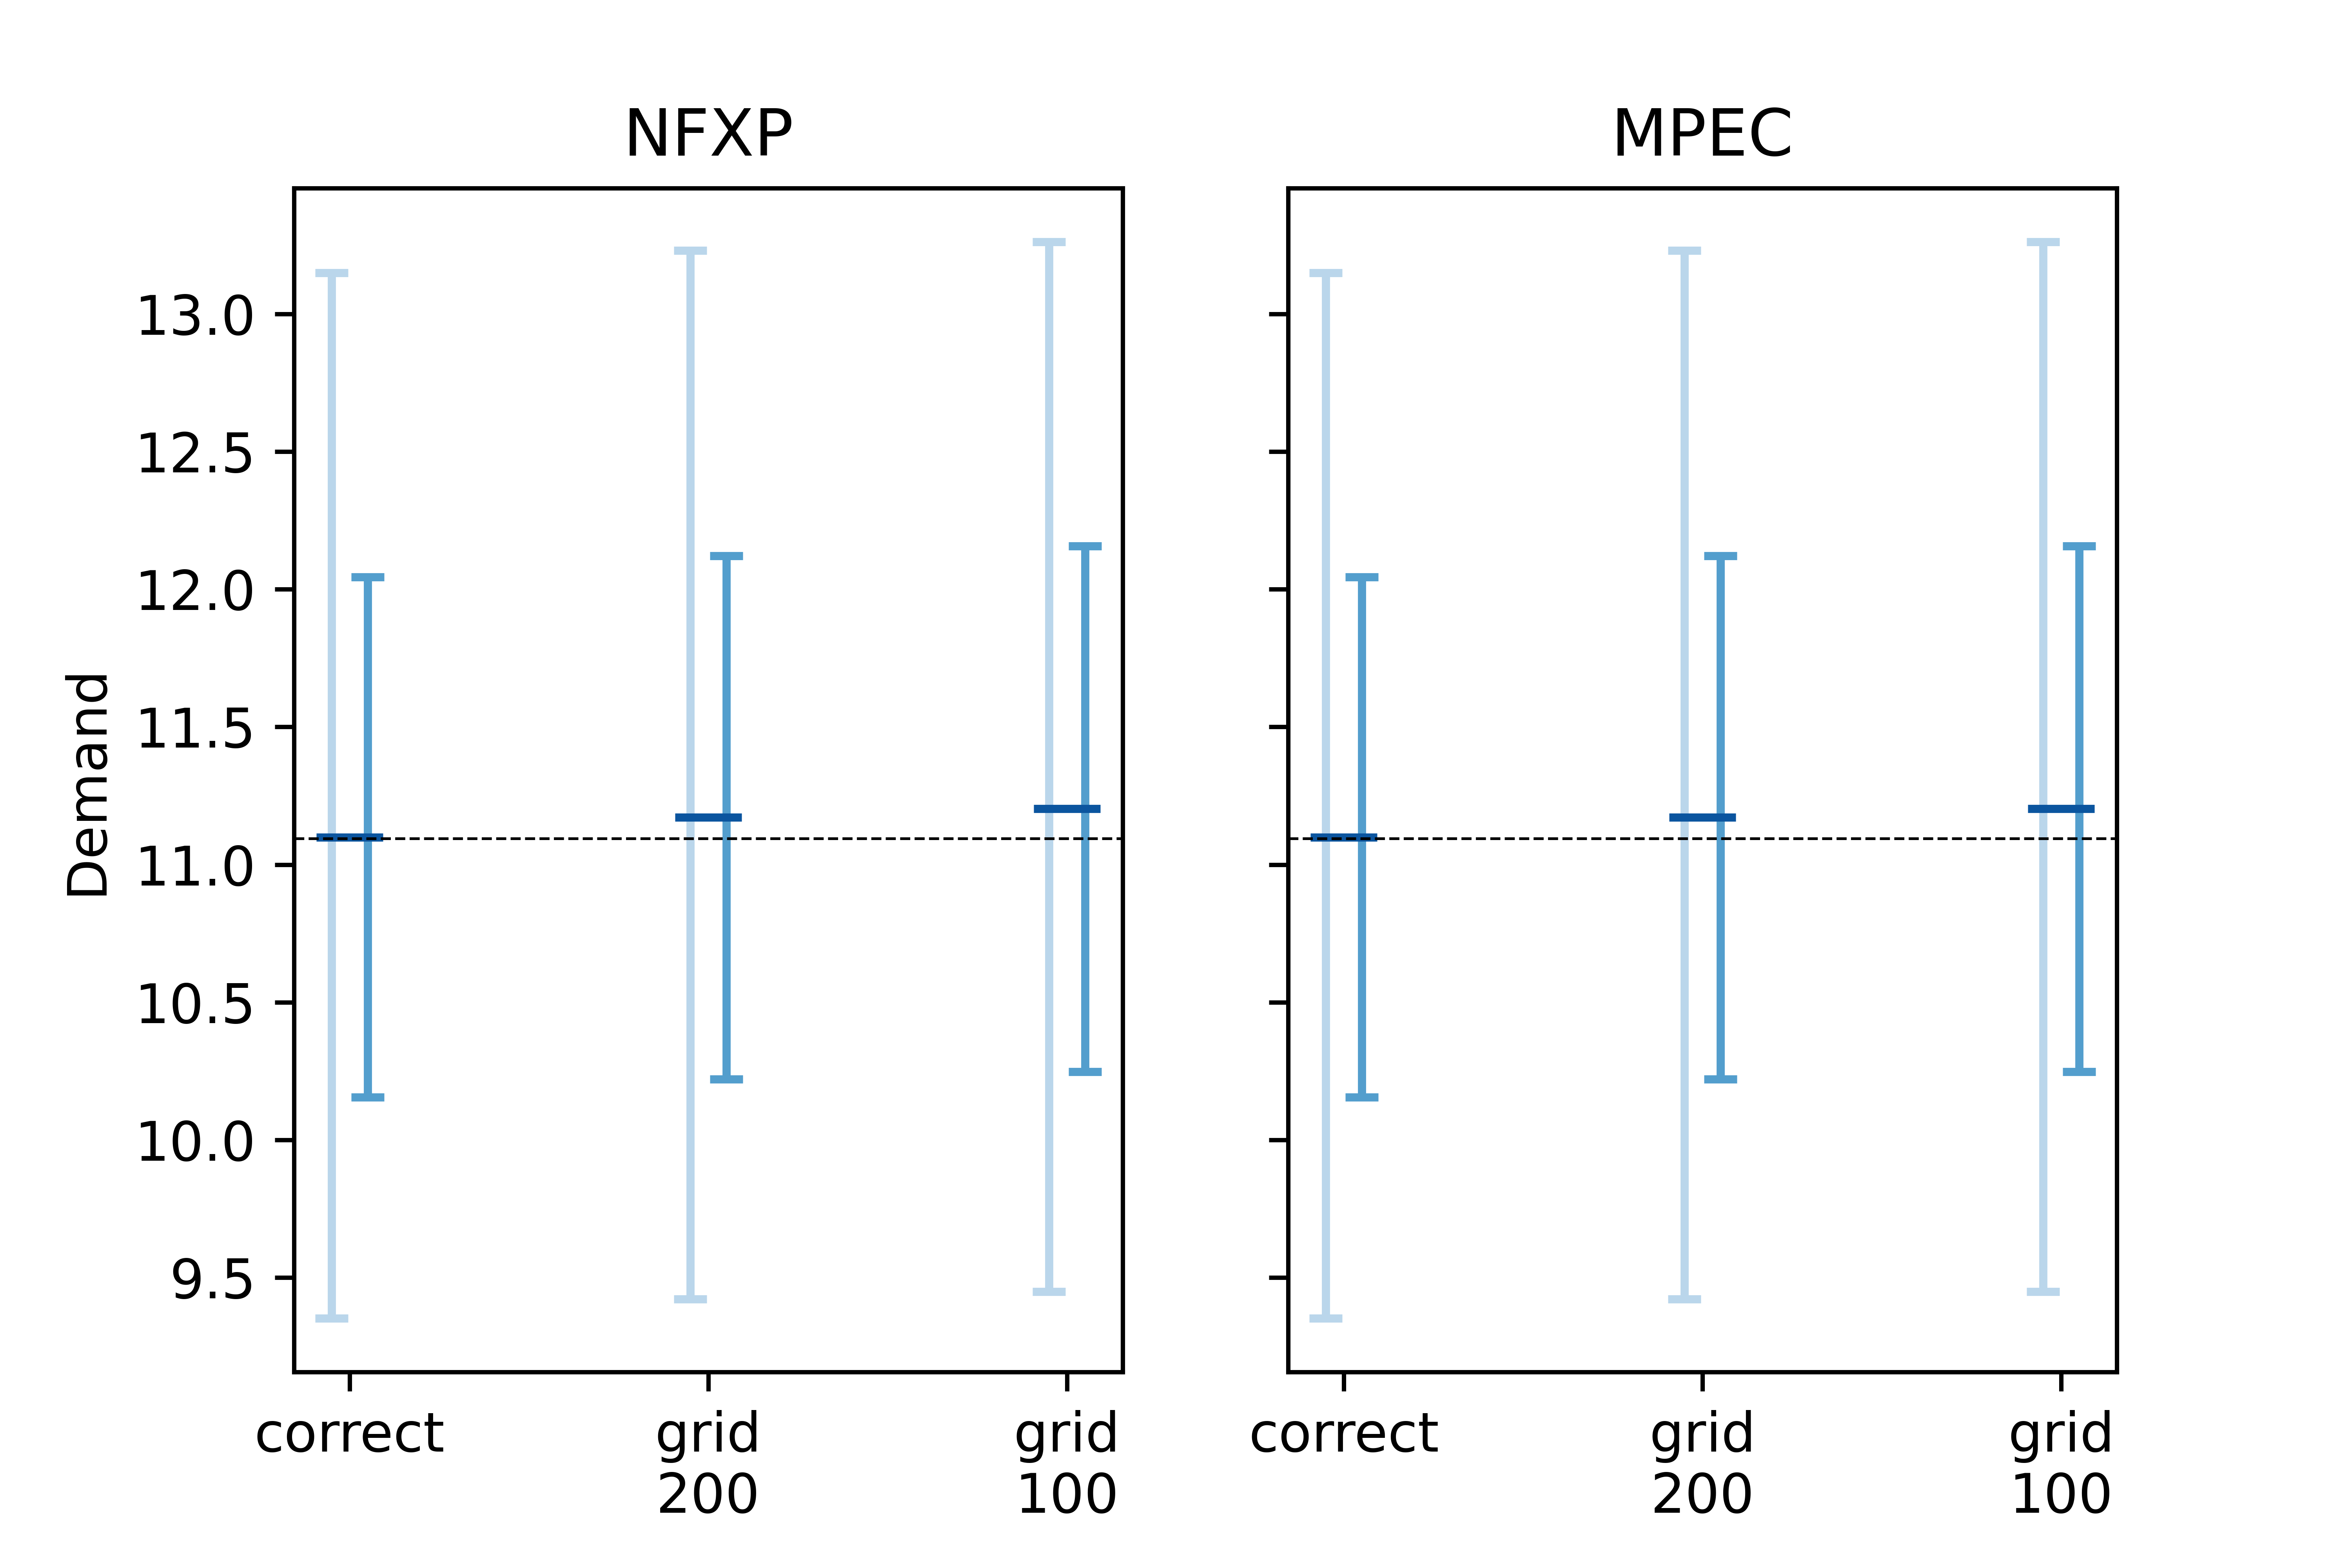
\includegraphics[scale=0.9]{../figures/figure_7.png}
	\label{figure7}
\end{figure}

After this singular view on the model dimension, we will repeat this for the numerical dimension. In Figure \ref{figure7} I split the grid size from the case that holds all information (400 grid points) in half twice, ending up with a grid size of 200 first and 100 second. This loss of information introduces a small downward bias in comparison to the correct specification. With my low number of Monte Carlo runs, this actually makes the prediction better when looking at the true QoI. Although it cannot be said with certainty from my setup but it is likely that with increasing runs this downward bias will persist ending up in estimates for lower grid sizes that will be below the true parameter. With certainty it can only be said that as the mean calculated in the correct specification is a consistent estimate of the true QoI, lowering the grid size is not generally beneficial.

In Figure \ref{figure8}, we conclude the partial view on the numerical dimension by adding numerical gradients as opposed to analytical ones. The rationale of adding this dimension is to observe how MPEC and NFXP react to the realistic assumption that the likelihood function is not differentiable. Both \cite{Su.Judd.2012} as well as \cite{Iskhakov.2016} utilize the build-in tool of automatic differentiation in the AMPL modeling language to obtain analytical derivatives of the likelihood function for MPEC. I abstract from this by supposing that there is no analytical derivative and hence it has to be approximated numerically. For this I rely on two-point finite differences. As can be seen in the figure, in the qualitative results of both MPEC and NFXP this numerical error does not make any difference in the estimates of the QoI irrespective of solely having this error or whether it is paired with decreasing grid size. This means that the estimates are the same for the displayed specifications regardless of whether numerical or analytical derivatives are applied.

\begin{figure}[!b]
	\caption{The QoI varying the Grid Size and the Gradients}
	\vspace*{-4mm}
	\centering
	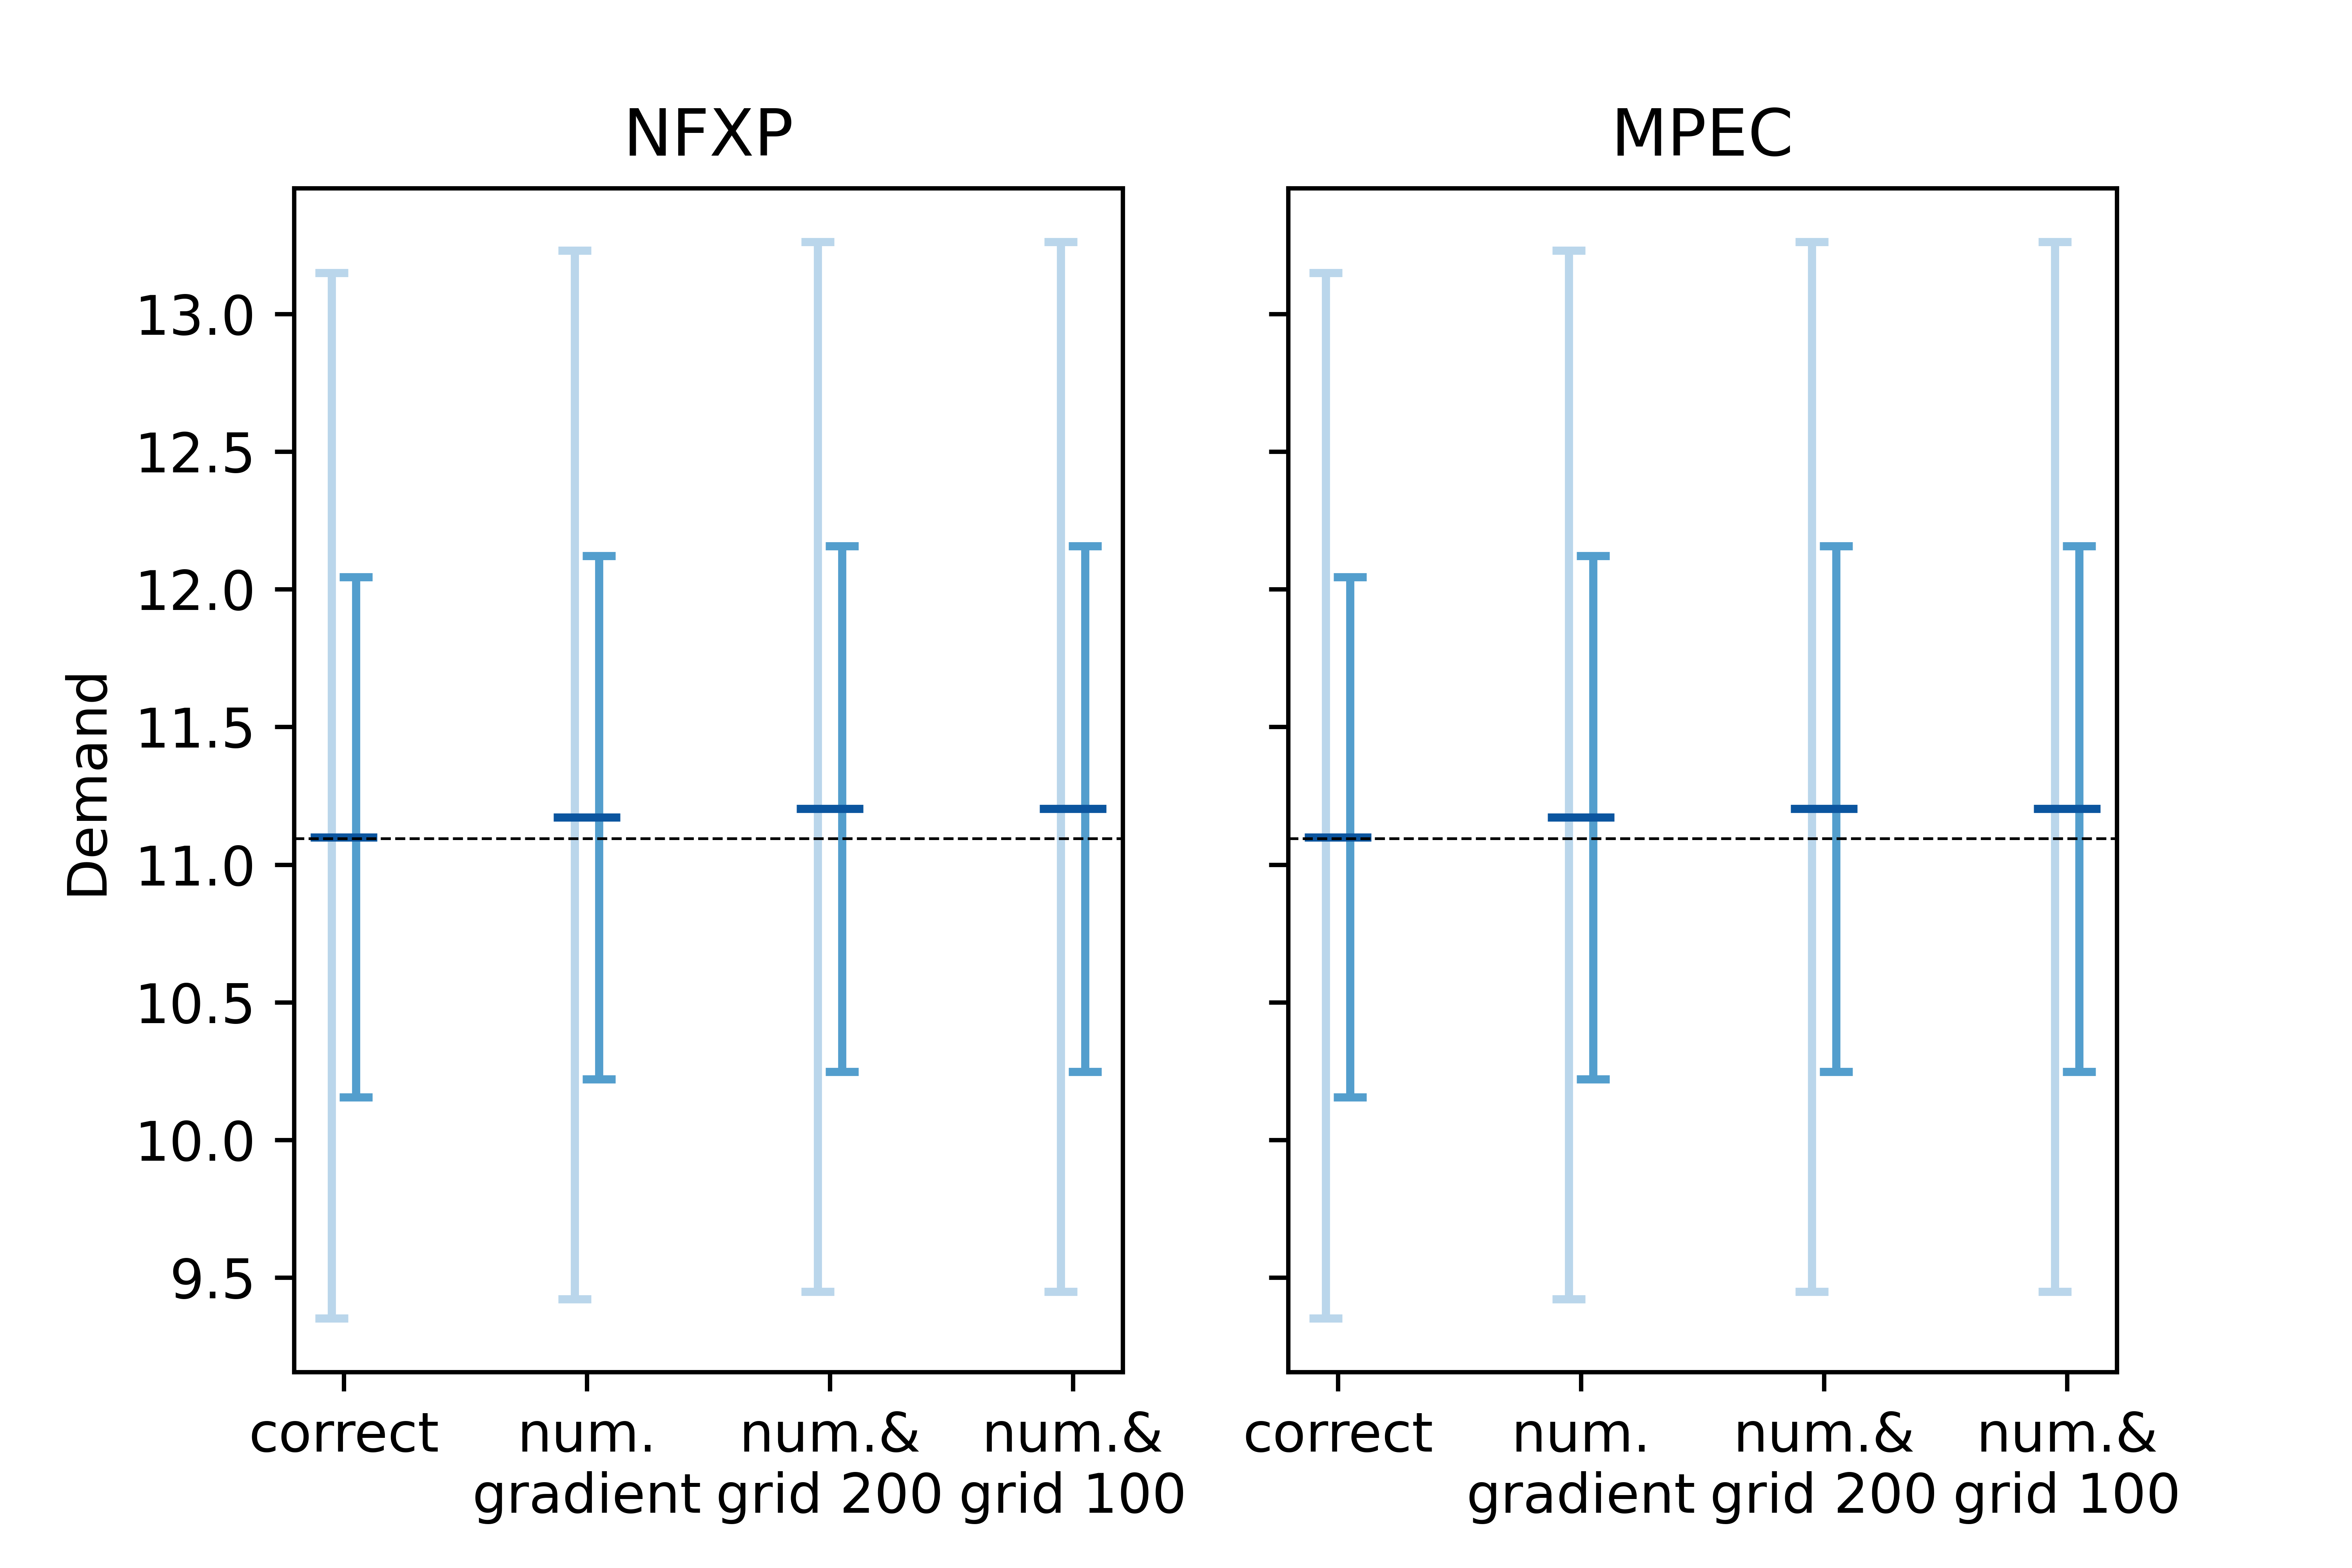
\includegraphics[scale=0.9]{../figures/figure_8.png}
	\label{figure8}
\end{figure}

When it comes to the quantitative comparison as done in \cite{Iskhakov.2016} there is a notable difference, though. Relying on finite differences comes with more function evaluations needed per major iteration of the solver. Per derivative evaluation of the solver the two-point finite difference approach makes two function evaluations per parameter. As there is a difference between MPEC and NFXP in the amount of derivative evaluations needed and of parameters, this translates into a different number of total function evaluations. When using IPOPT for MPEC it is necessary to supply the augmented log likelihood with its gradient as well as the constraints with its Jacobian. Assuming the grid size to be 400 and the cost function to be linear, one derivative of the likelihood function comes with $402 \times 2$ likelihood function evaluations as well as $400 \times 2$ constraint evaluations. In the case of the NFXP this is less daunting. As there are only two parameters and solely the gradient of the likelihood function is required, one gradient evaluation results in two additional function evaluations. A single function evaluation is more costly, though, in the case of the NFXP as each time the economic model has to be solved. In the Rust model this means that with high precision a fixed point has to be calculated, while in the case of MPEC the function is simply evaluated at a given point. This tradeoff determines whether MPEC or the NFXP is more efficient when using numerical derivatives and clearly this also depends on the grid size as it affects the dimension of the fixed point for the NFXP and the number of parameters for MPEC. This tradeoff clearly has an effect on which models might be more efficiently estimated with one or the other approach which is what I examine in appendix B with the class of Eckstein-Keane-Wolpin models.

When comparing the correctly specified to the same model but with numerical derivatives, for MPEC the number of likelihood function evaluations increases from on average roughly 23 to about 8540 (not taking into account the rising number of constraint evaluations). The amount of time needed on average is around seven times as high. For the NFXP the likelihood function comes from 13 on average and increases to approximately 39.\footnote{The 39 function evaluations are solely an approximation as estimagic does not allow to give out the total number of function evaluations including those needed for the numerical derivatives. As the L-BFGS-B roughly needs as many gradient evaluations as function evaluations, the total number of function evaluations is approximated by $13+13 \times 2$.} At the same time, this affects the number of contraction and N-K iterations. They rise on average from 285 to 1080 and from 77 to 287. The CPU time needed for the NFXP with numerical derivative is only twice as high as is the case with analytical gradient. Clearly, this tradeoff between MPEC and NFXP depends heavily on the efficient solving of the economic model as well as the capability of solving the problem with a low number of gradient evaluations.

\begin{figure}[!b]
	\caption{Distribution of the QoI}
	\vspace*{-4mm}
	\centering
	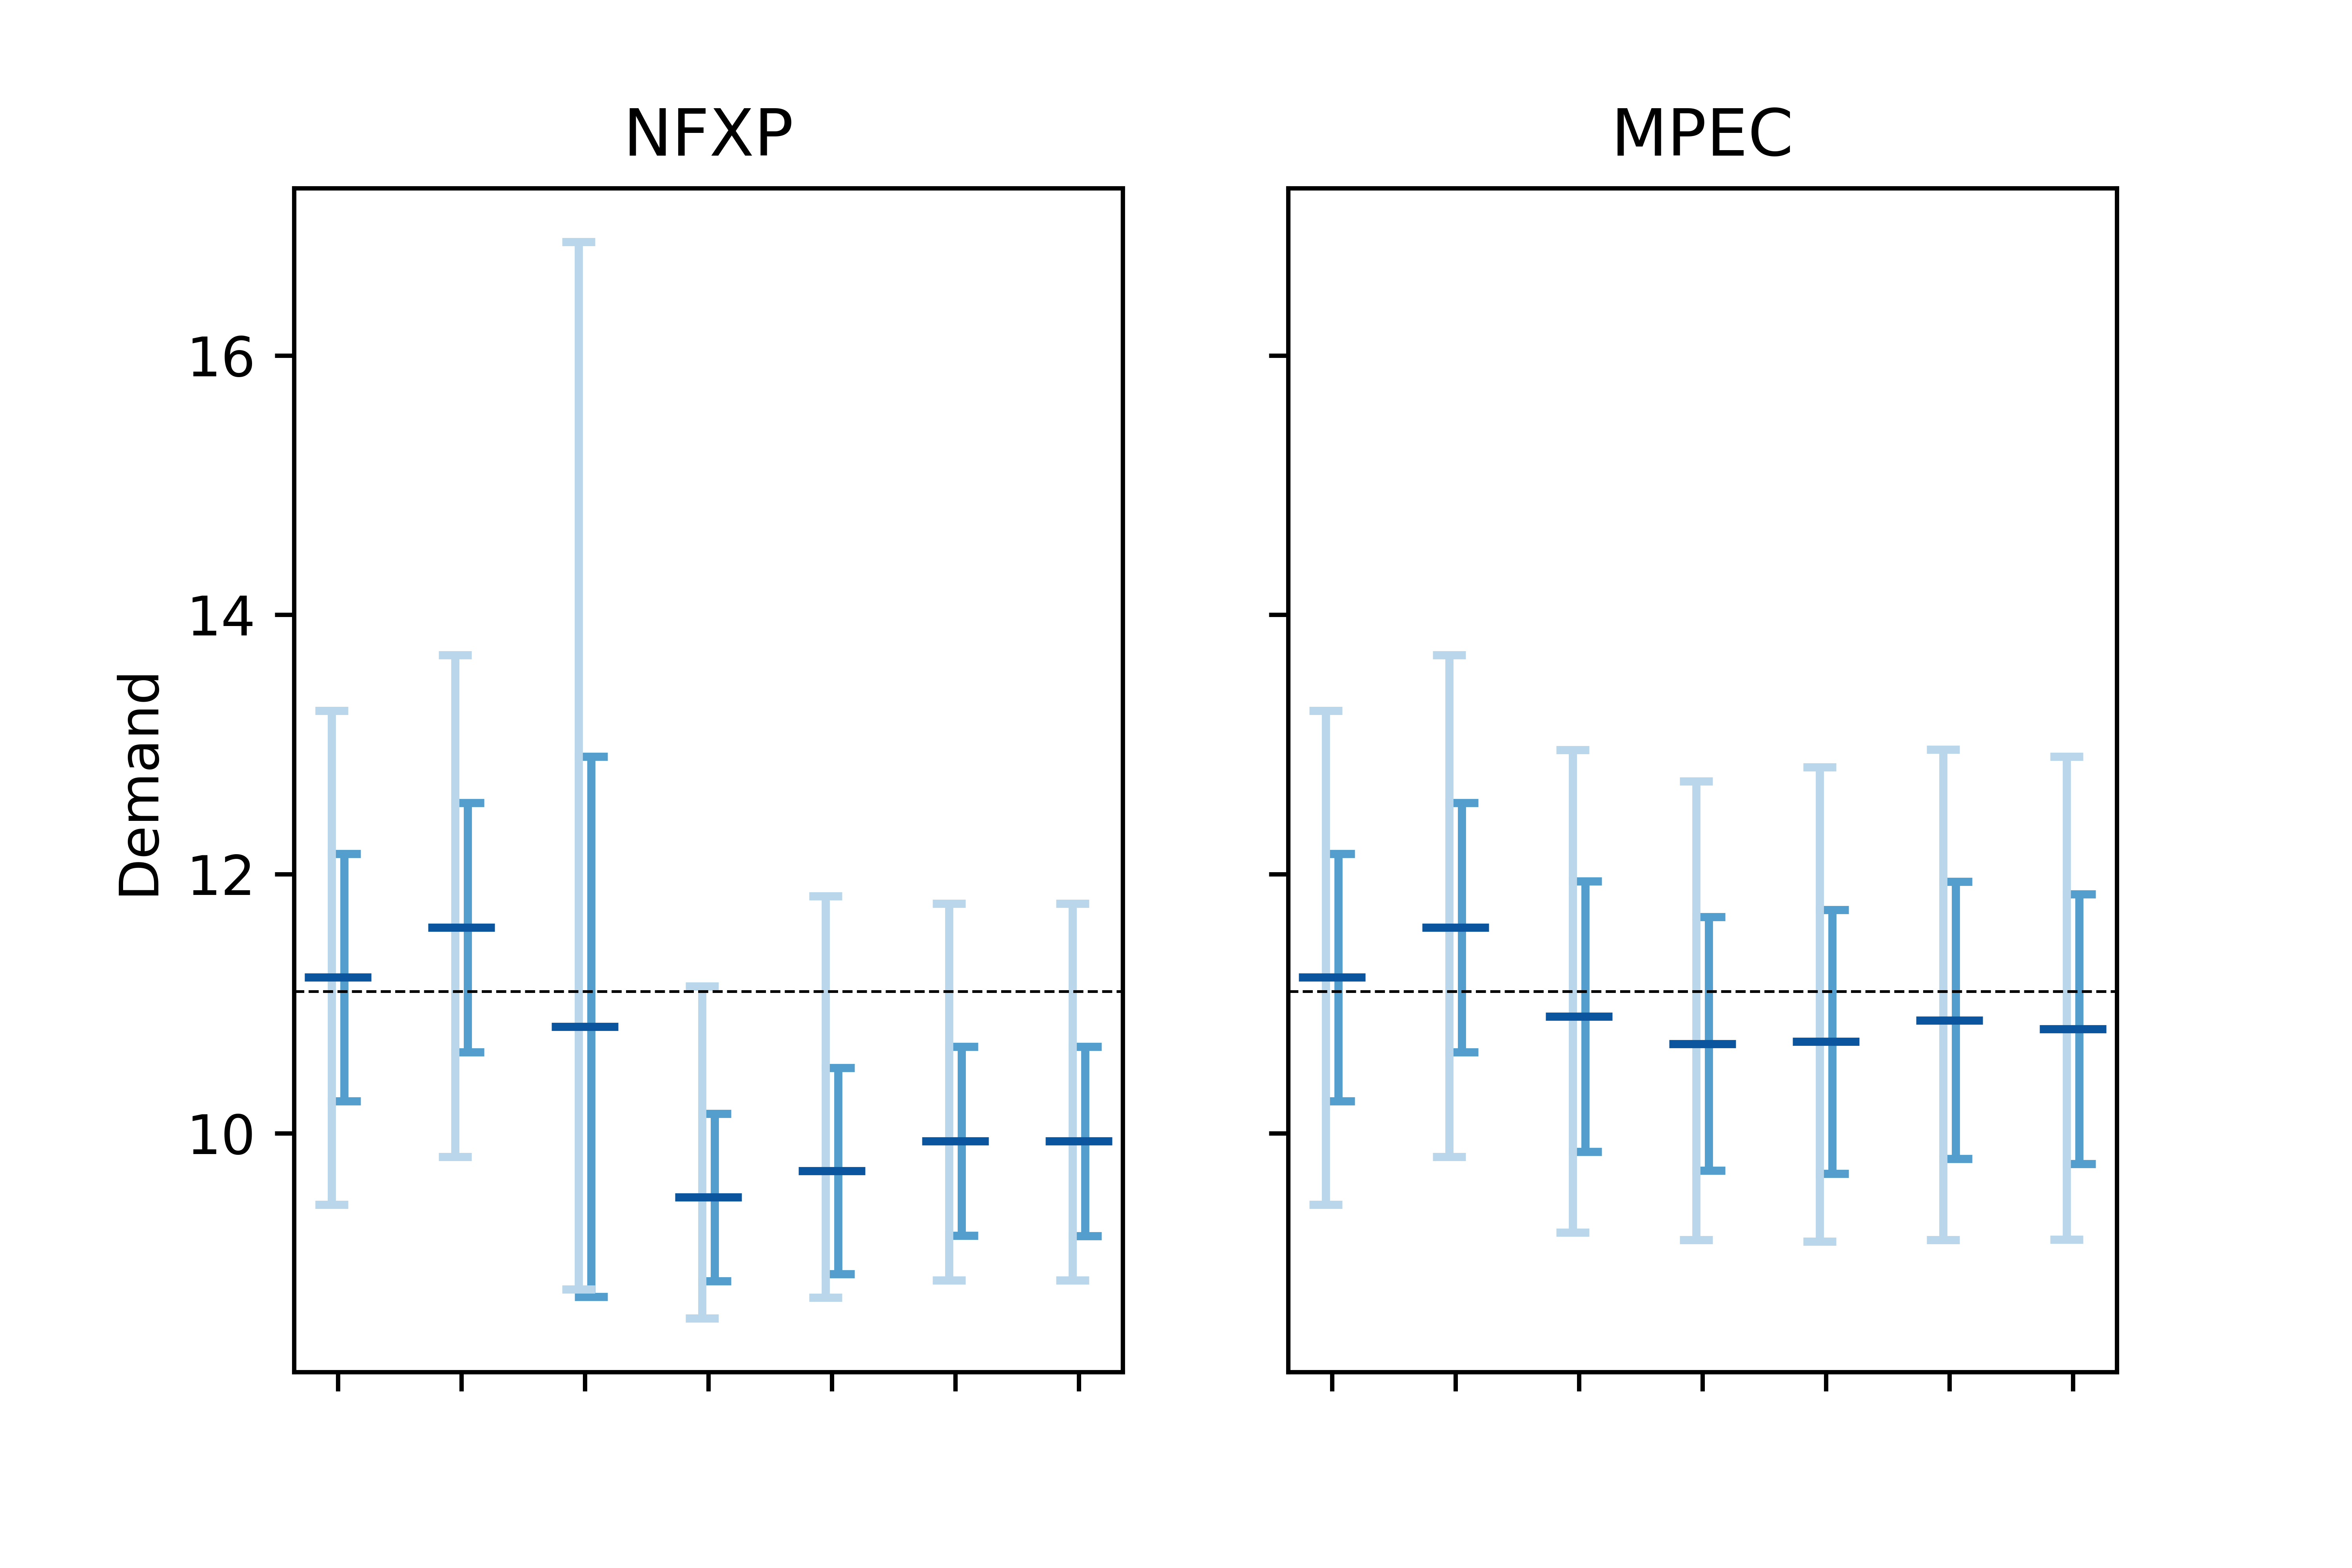
\includegraphics[scale=0.9]{../figures/figure_9.png}
	\label{figure9}
\end{figure}

When comparing how those statistics change from using numerical derivatives with grid size 400 to lower grid size, it becomes apparent that for MPEC this makes a large difference. The number of likelihood function evaluations roughly halves when dividing the grid size by two. The CPU time needed is every time roughly divided by seven. For the NFXP the number of contraction and N-K steps stays roughly constant while the CPU time still is divided by three to four each time. When using finite-difference numerical derivatives the NFXP seems to be superior in my setting in regard of the quantitative efficiency due to the lower dimensionality of the problem it solves.

From an uncertainty perspective, in this partial view the use of numerical derivatives does not have an effect on the QoI. However, the numerical error introduced by lowering the grid size does shift some key characteristics of its distribution downwards.

In Figure \ref{figure9}, which concludes this section, I introduce a possible sequence of different specifications coming from the correctly specified model on the left to a model in which every possible dimension is wrongly specified on the right. As a matter of fact, the first four specifications are those from Figure \ref{figure6} in which I first incresae $\beta$ and then additionally allow for more flexibility in the cost function. From four to five I add numerical gradients which in the following specifications is combined with decreasing grid size. In the last sepcification we hence end up with the most extreme case in which the cost function is assumed to be cubic, $\beta$ equals to 0.985, numerical derivatives are used and the grid size amounts to 100. When facing already some misspecification, the switch from analytical derivatives to numerical ones has a small effect for MPEC this time. The mean shifts from $10.873$ to $10.804$ as well as the other statistics move downwards. As the qualitative results are only calculated for runs that successfully converged, this can be explained by a lower convergence rate of MPEC which is around 80 percent. From that on both approaches incur an increasing downward bias with decreasing grid size. Again the rate of convergence of MPEC is ranging between 66 and 83 percent. The distribution of MPEC seems to maybe shift a bit in the sense that less probability mass is above twelve and more at the lower end of the estimates. For the NFXP it is interesting to see that confidence and standard deviation intervals react to the change in grid size as well. Those observations suggest that there might be more subtle changes in the uncertainty of the QoI when looking at its whole distribution. This will be done in the next section where I will bring in a comparison of all possible 36 specifications.

\subsubsection{The Full Perspective}

In the real world when having only one data set at hand from which we do not know the data generating process we lack the information of how our model estimation actually performs. The true QoI is unknown as is the the true mathematical model. The computational model is surely an imperfect approximation of the mathematical one and there is no direct guidance on which specification of the demand model is actually the most accurate. In this setting, the more important it becomes to obtain as much information as possible on how sensitive the model reacts to certain misspecifications in which ever dimension of error. This is where uncertainty quantification is positioned and where the previously mentioned sub field \textit{sensitivity analysis} operates in regard of parameter uncertainty. As \cite{Oberkampf.2010} argue, as much information as possible should be incorporated into the process of obtaining the QoI by propagating this information through the model and making it available to policy makers.

In my simulation setup I am able to actually make a qualitative comparison of different specifications and make a stance on how sensitive the model prediction replies to a certain setting. In Figure \ref{figure10}, I now draw from a common measure for predictive performance which is the mean squared error (MSE) that I calculate for the estimated QoI per specification and approach. This yields an readable overview of which specifications and consequently which error the model is more or less reactive to. We can see that the model responds strongly do whether NFXP or MPEC is used to obtain the parameter distribution that is propagated through the model. Further the choice of the cost function has a visible effect, too, increasing the MSE with more flexibility in the cost function in comparison to linear cost. The reaction to the grid size appears to be case specific while the tradeoff between numerical and analytical gradient is only slightly observable. It is more pronounced, though, for MPEC. The increase in $\beta$ leads to less prediction precision with linear costs but the converse with other cost functions. At this point, it should be mentioned that in a few cases I observe the same phenomenon as \cite{Dong.Hsieh.Zhang.2017} did considering the NFXP. As explained before already, they find that the NFXP in some cases visits structural parameter guesses that causes the model solving procedure to fail. This is due to its separation of the estimation procedure into two loops. In my simulation it happens as well four times that the N-K step cannot be calculated causing the NFXP to not converge while MPEC does. While this can be healed through back switching to contraction steps in the NFXP, it is still worth mentioning that I can confirm their finding in my setting.


\begin{figure}[!b]
	\caption{Distribution of the QoI}
	\vspace*{-4mm}
	\centering
	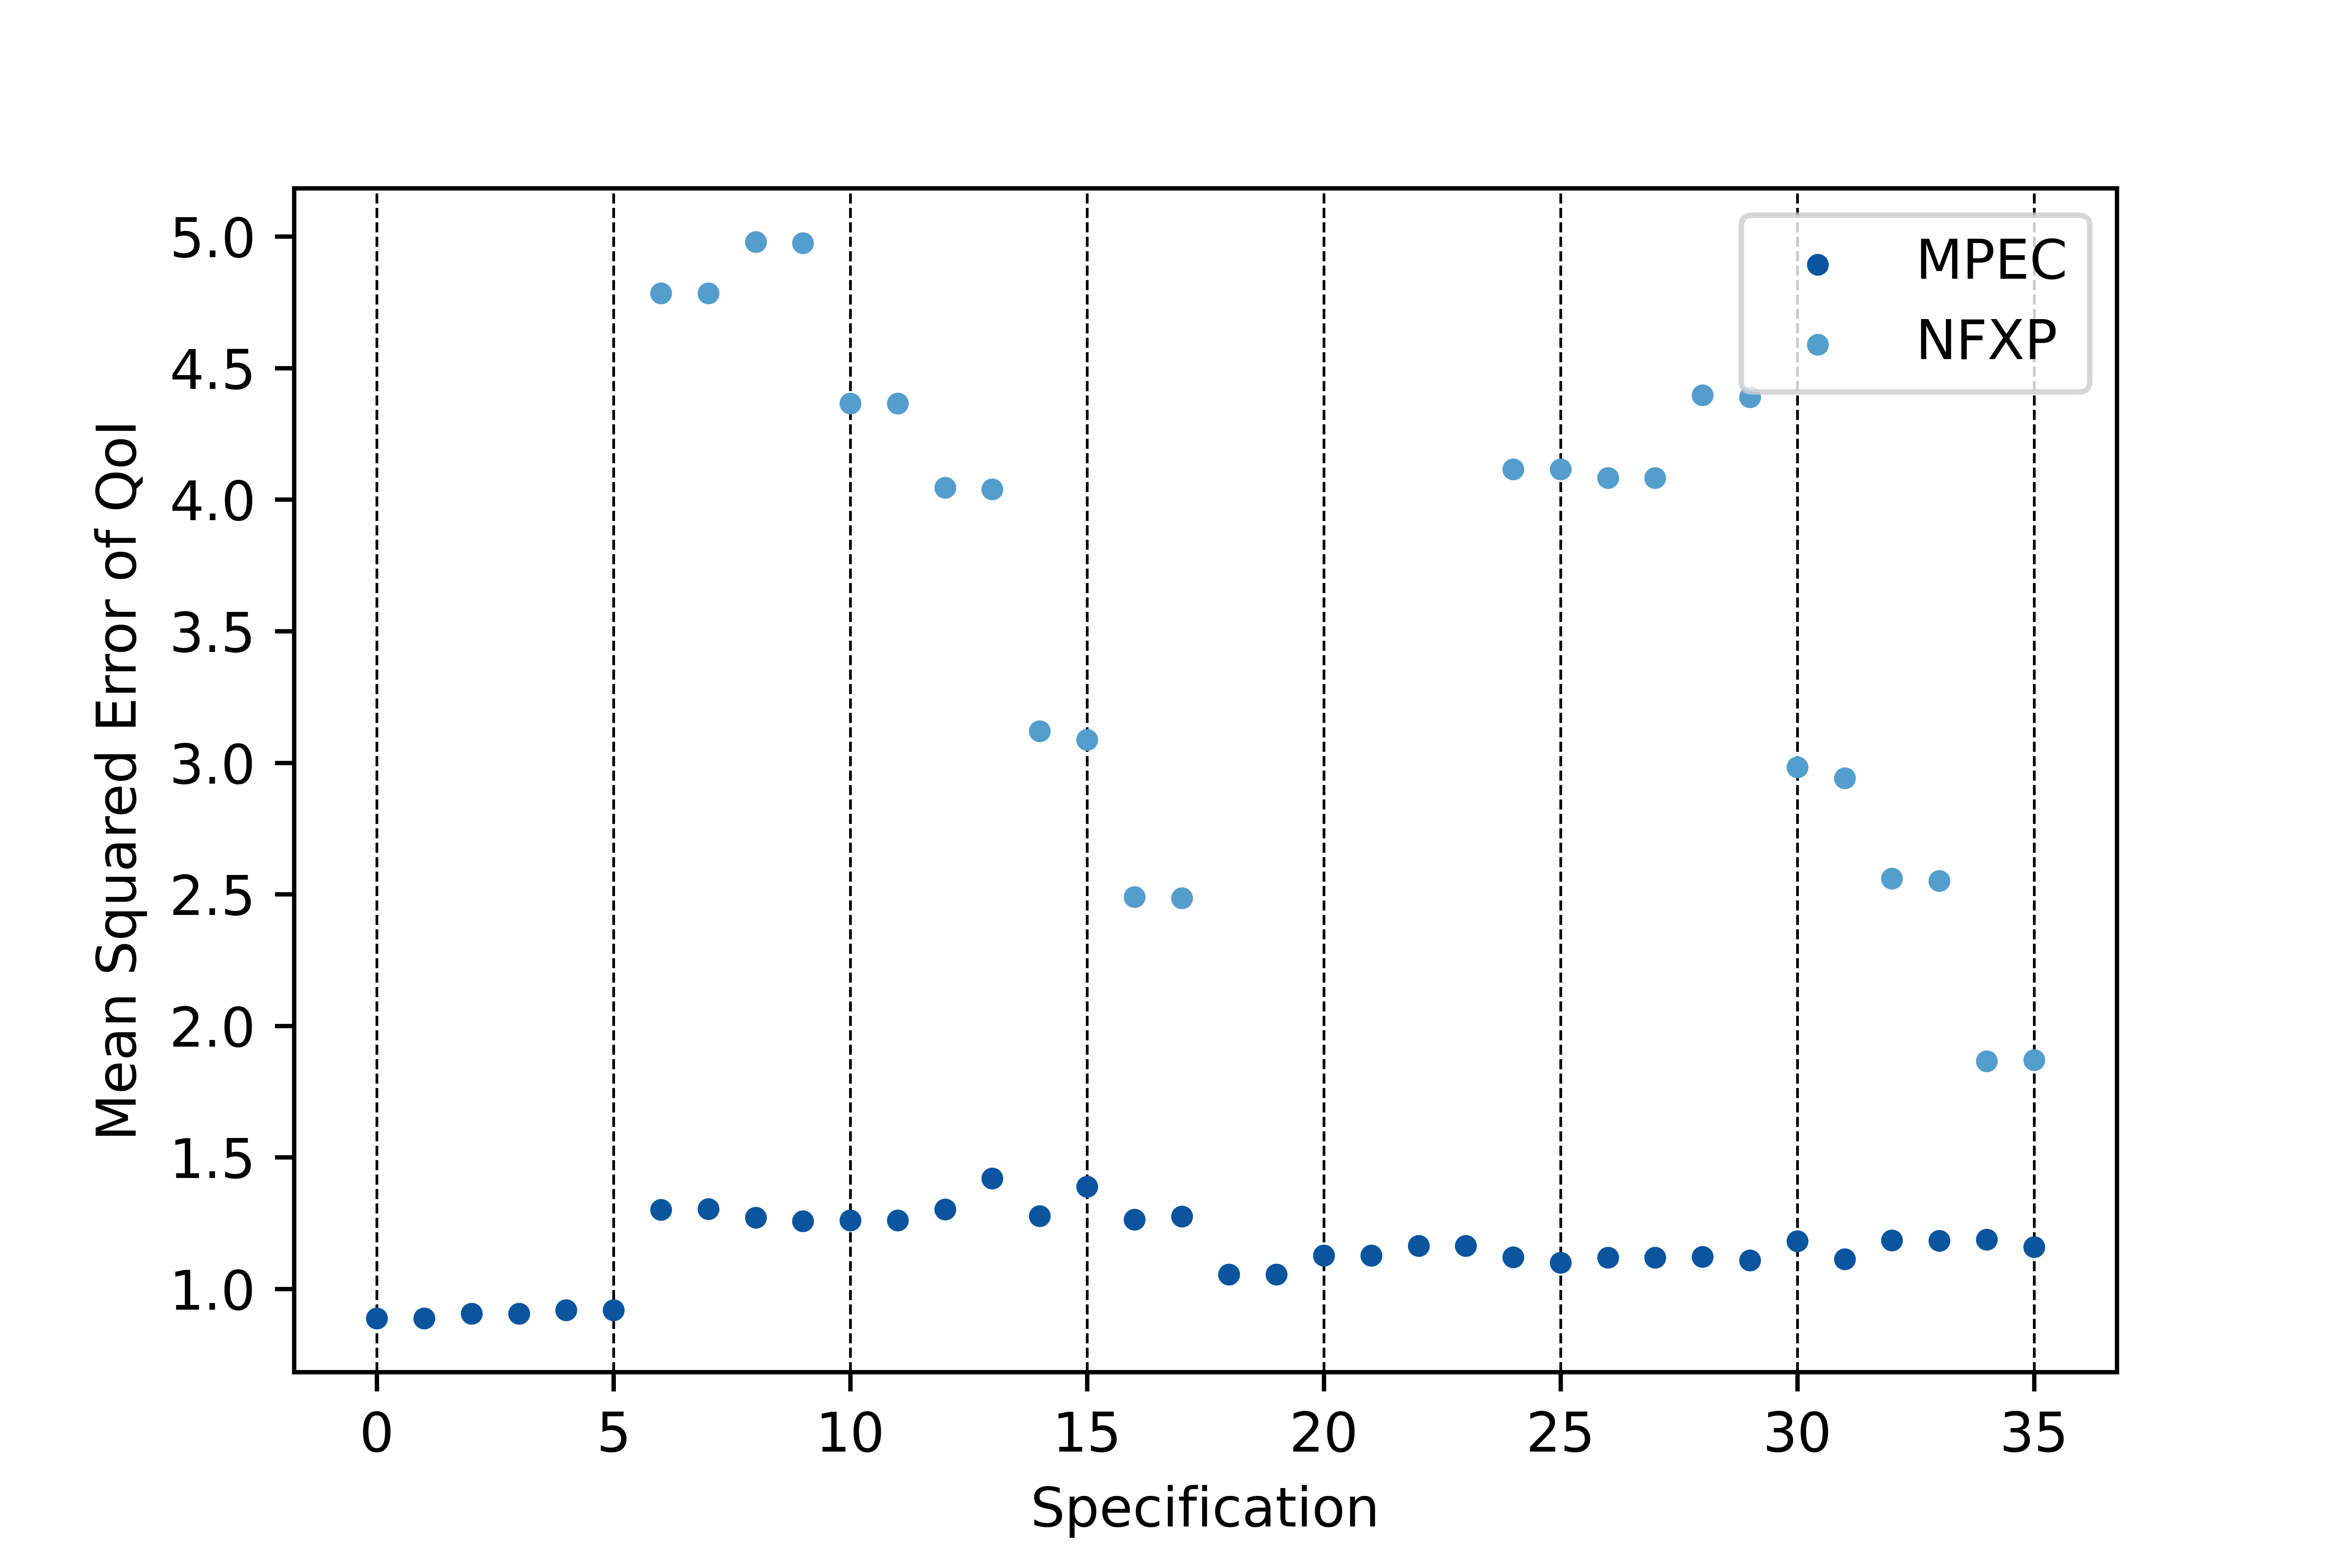
\includegraphics[scale=0.9]{../figures/figure_10.png}
	\label{figure10}
\end{figure}


I conclude this section with Figure \ref{figure11} which loosely refers to the visualizations in \cite{Oberkampf.2010}. For the case of having used MPEC across all specifications, I plot the resulting distributions of the QoI for each specification. In the first window the probability density function and in the second the cumulative probability function. What all have in common is that they are bell shaped while being more or less left-skewed. The correctly specified model has its peak slightly to the left of the true parameter while the mean is actually slightly above it which is due to some strong overestimations of the QoI. I further marked in slightly lighter blue the two distributions that frame the others to visualize in which range the distributions are. The left frame corresponds the specification in which I combine the true $\beta$ with cubic cost, a grid size of 100 and numerical derivatives. The right frame is represented by the true specification with the only difference that $\beta$ is equal to 0.985. All other specifications are depicted by the often overlapping light blue/gray curves. It can be seen that the resulting distributions can be roughly split up into three groups. The group on the very far right consists of all specifications in which the linear cost function is combined with an increased $\beta$. This is irrespective of grid size and choice of derivative and seems to shift the distribution of the correctly specified model to the right. The second group which is around the correctly specified model is made of the those specifications that rely on a linear cost function paired with the true $\beta$. The rather large group of distributions on the left are now consisting of all those specifications with either quadratic or cubic costs irrespective of grid size and/ or numerical derivatives. This group is slightly split into two as there are two bigger bundles with a small gap in between. The right hand side again are those specifications that use the increased $\beta$ of 0.985. So, in general, the increased $\beta$ shifts the existing distribution to the right. In general, the far left distributions that are defined by a more flexible cost function actually change the distribution in the QoI to a more left-skewed one. In the window below the previously explained patterns are equally visible with the probability distribution function.

The whole figure conveys three key messages. First, by propagating a reasonable distribution of parameter estimates through the demand function model we can uncover the probabilistic uncertainty around the QoI. Second, we can detect across a specific range which model and numerical errors in the calibration procedure and the modeling of the demand function translate into different estimated parameters which in turn result in a range of possible distributions of the QoI. Third, this range can be now used to uncover which errors affect the uncertainty in the QoI in which way. This range serves as additional information for policy makers that accounts for more than just simple variation in the parameter estimates stemming from estimation with sample data based on a single specification of the mathematical and computational model.

For an entirely comprehensive representation of my simulation, one would complement the figure by the same using the NFXP. This is Figure \ref{figure13} which can be found in the appendix. As can already be guessed, the resulting distributions when using the NFXP look very different across specifications. Let us put ourselves in the position of having performed my previous study with one real data set from which we bootstrapped 249 other data sets. Assume that we would have, hence, obtained my results using real data and without knowledge about the data generating process and therefore the true value of the QoI. If we had only estimated the data sets with the NFXP and flexible cost functions (the two blocks of distributions that are left-skewed at the very far left of ), this would have resulted in an entirely different distribution of the QoI than with other cost functions. A policy decision solely on this would be very much flawed. If the whole Figre \ref{figure13} was given the way it is now, the policy decision would be far more difficult to make as the range of possible distributions is large. But at the same time, this uncertainty can be incorporated and accounted for in policy which makes it more informed an robust. Having the knowledge about results from MPEC would even further enhance possible policy as has been established in this thesis that the qualitative results of MPEC and NFXP can systematically differ under certain circumstances (even after extensive robustness checks regarding solver, tolerances and fixed point setup in the NFXP). While the uncertainty quantification as done in my thesis is computationally expensive and might not be feasible for every model, there might ways to use surrogate models with different model and numerical errors together with existing global sensitivity techniques. In general, an uncertainty quantification of an economic model should be aimed for and given as an additional information to policy makers. This can further provide valuable information for researchers themselves to improve the model or calibrate it. It thus can also be beneficial for empiricists when later performing model averaging or model selection to improve the model predictions.

\begin{figure}[H]
	\caption{Distribution of the QoI}
	\vspace*{-4mm}
	\centering
	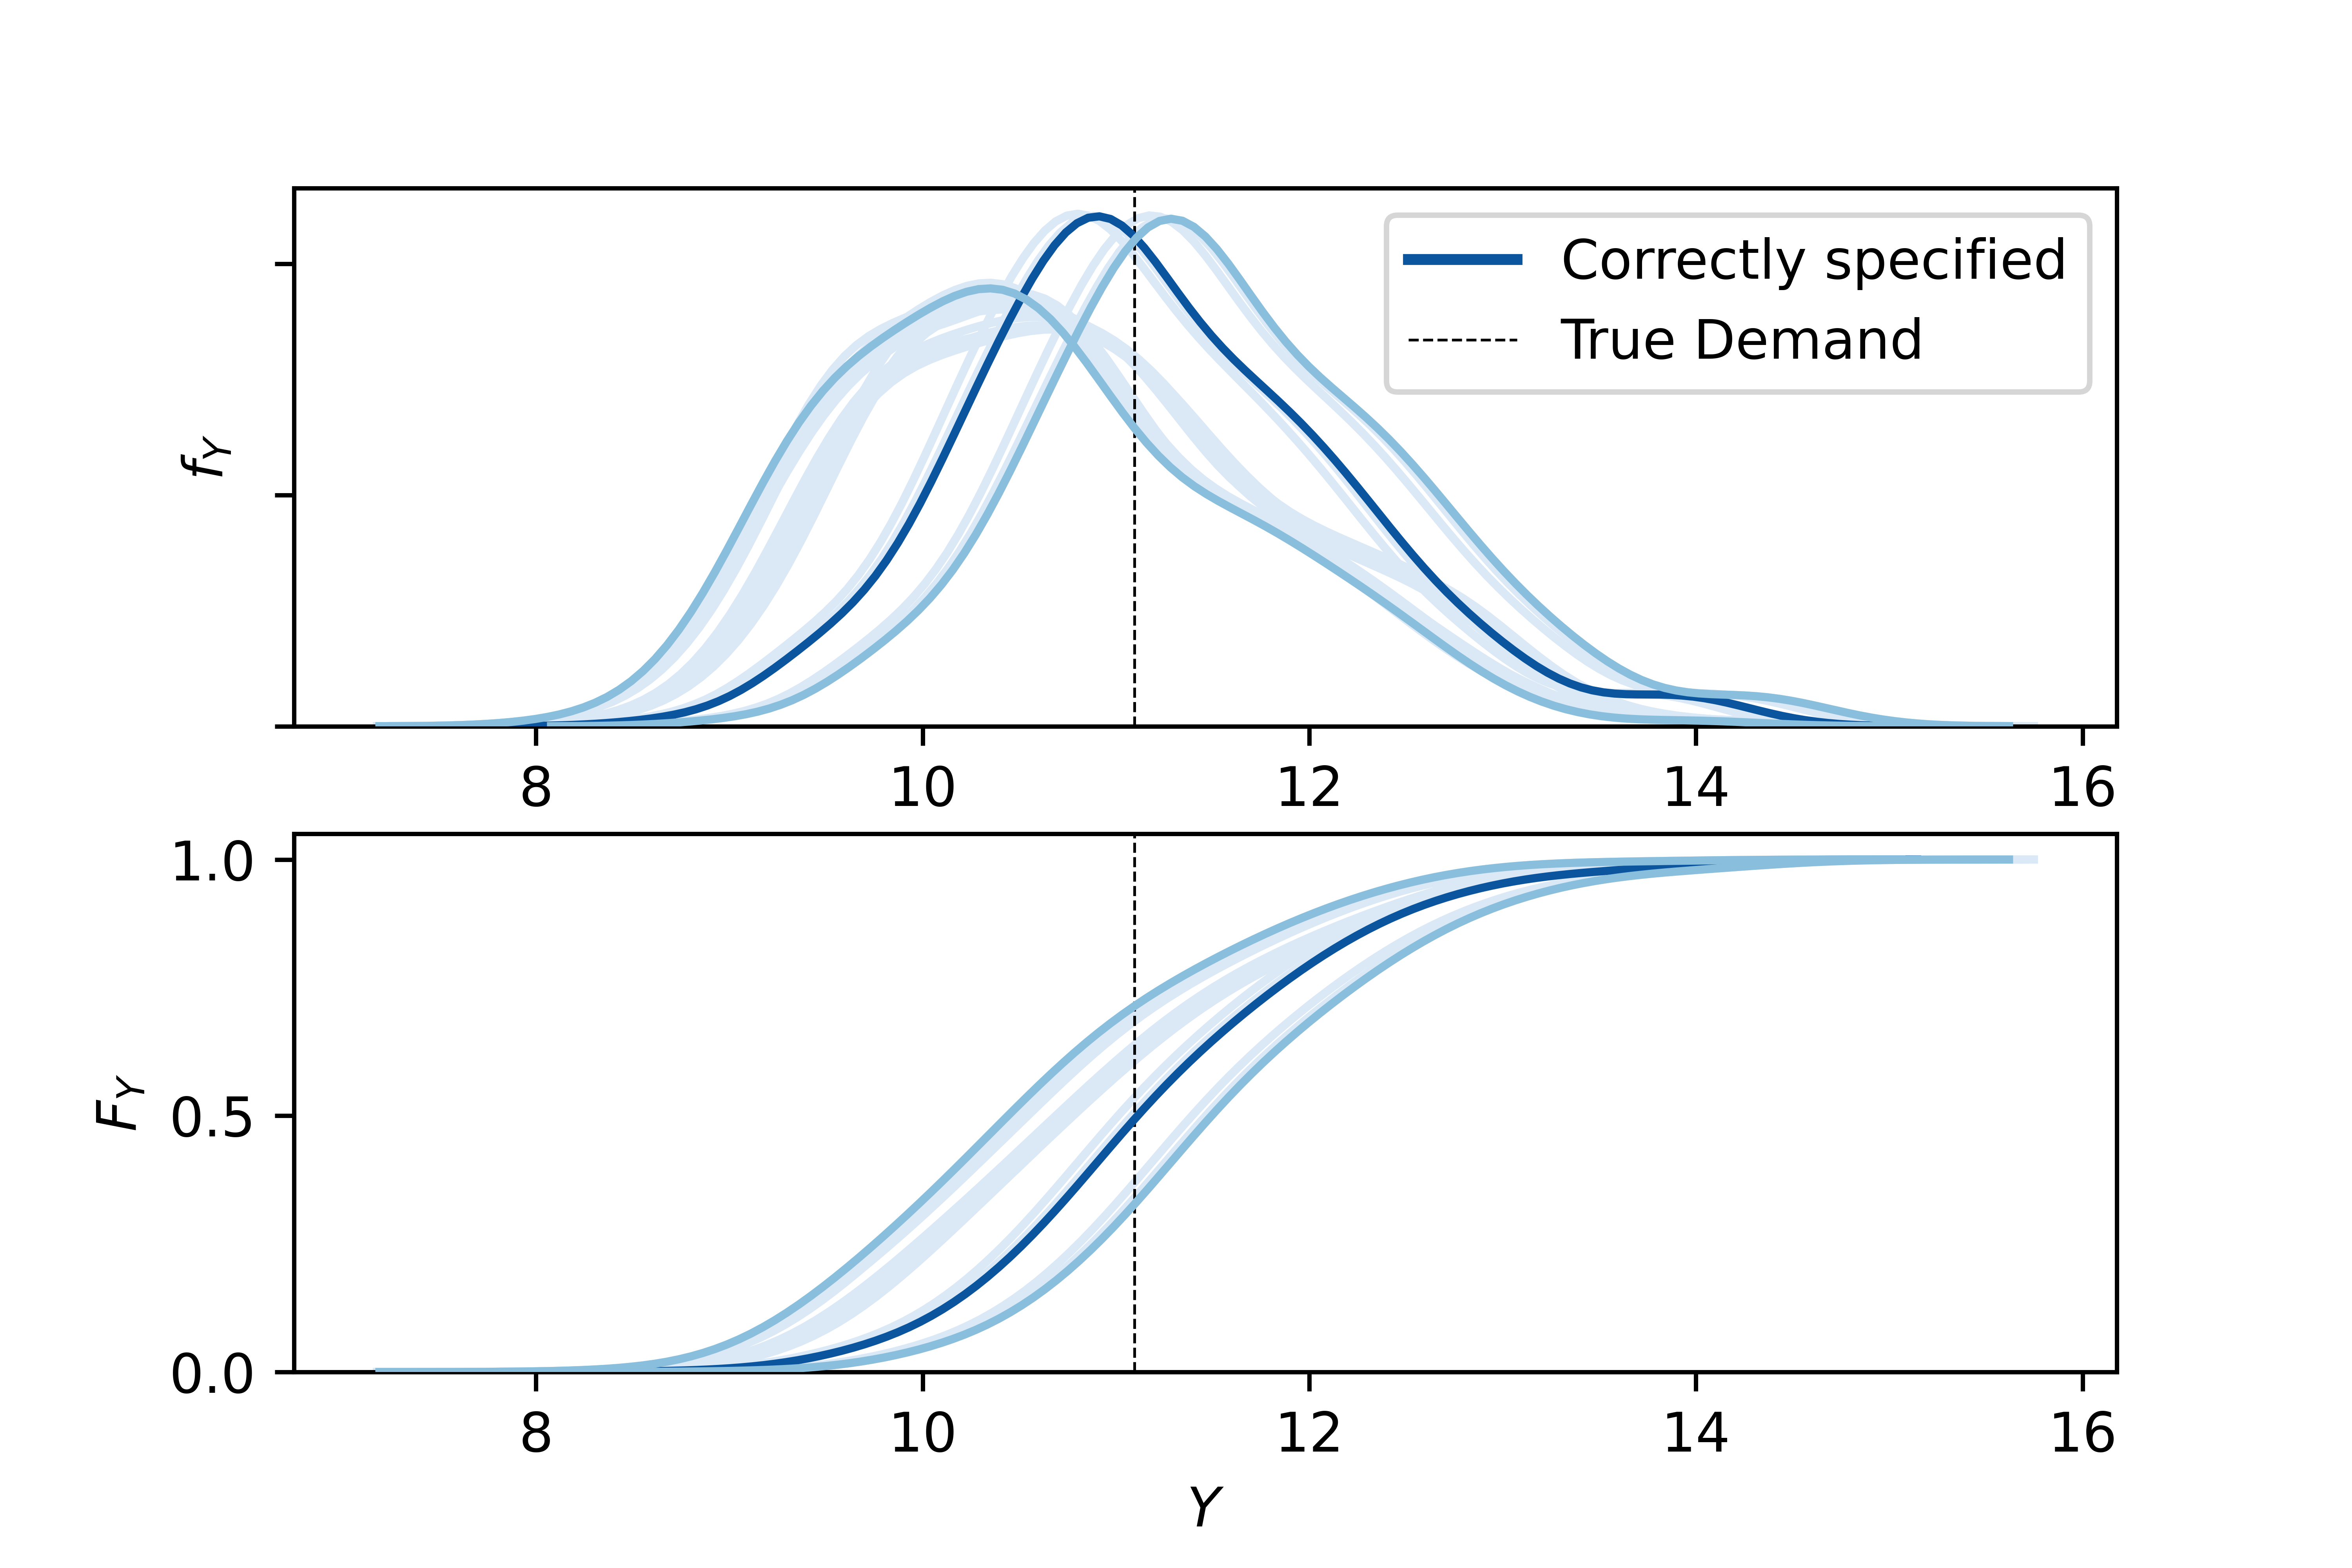
\includegraphics[scale=0.9]{../figures/figure_11.png}
	\label{figure11}
\end{figure}
